\section{Estimating the optimal vocabulary size}
\label{sec:estimation}

In this section, we describe three complementary approaches to estimate the optimal vocabulary size.



\subsection{Approach 1: Estimating power laws via IsoFLOPs}
\label{sec:isoflops}

We define 6 groups of models with $N_{\rm nv}$ ranging from 33M to 1.13B. Within each group, we solely vary the vocabulary size $V$ from $4K$ to $96K$, and evaluate different models under the same FLOPs budget.  We evaluate the normalized loss $\mathcal{L}_u$ on a held-out validation dataset. This approach allows us to directly answer the question: For a given FLOPs budget, what is the optimal allocation to non-vocabulary parameters, vocabulary parameters, and training data?

\begin{wrapfigure}{l}{0.5\textwidth}
\centering
\vspace{-4mm}
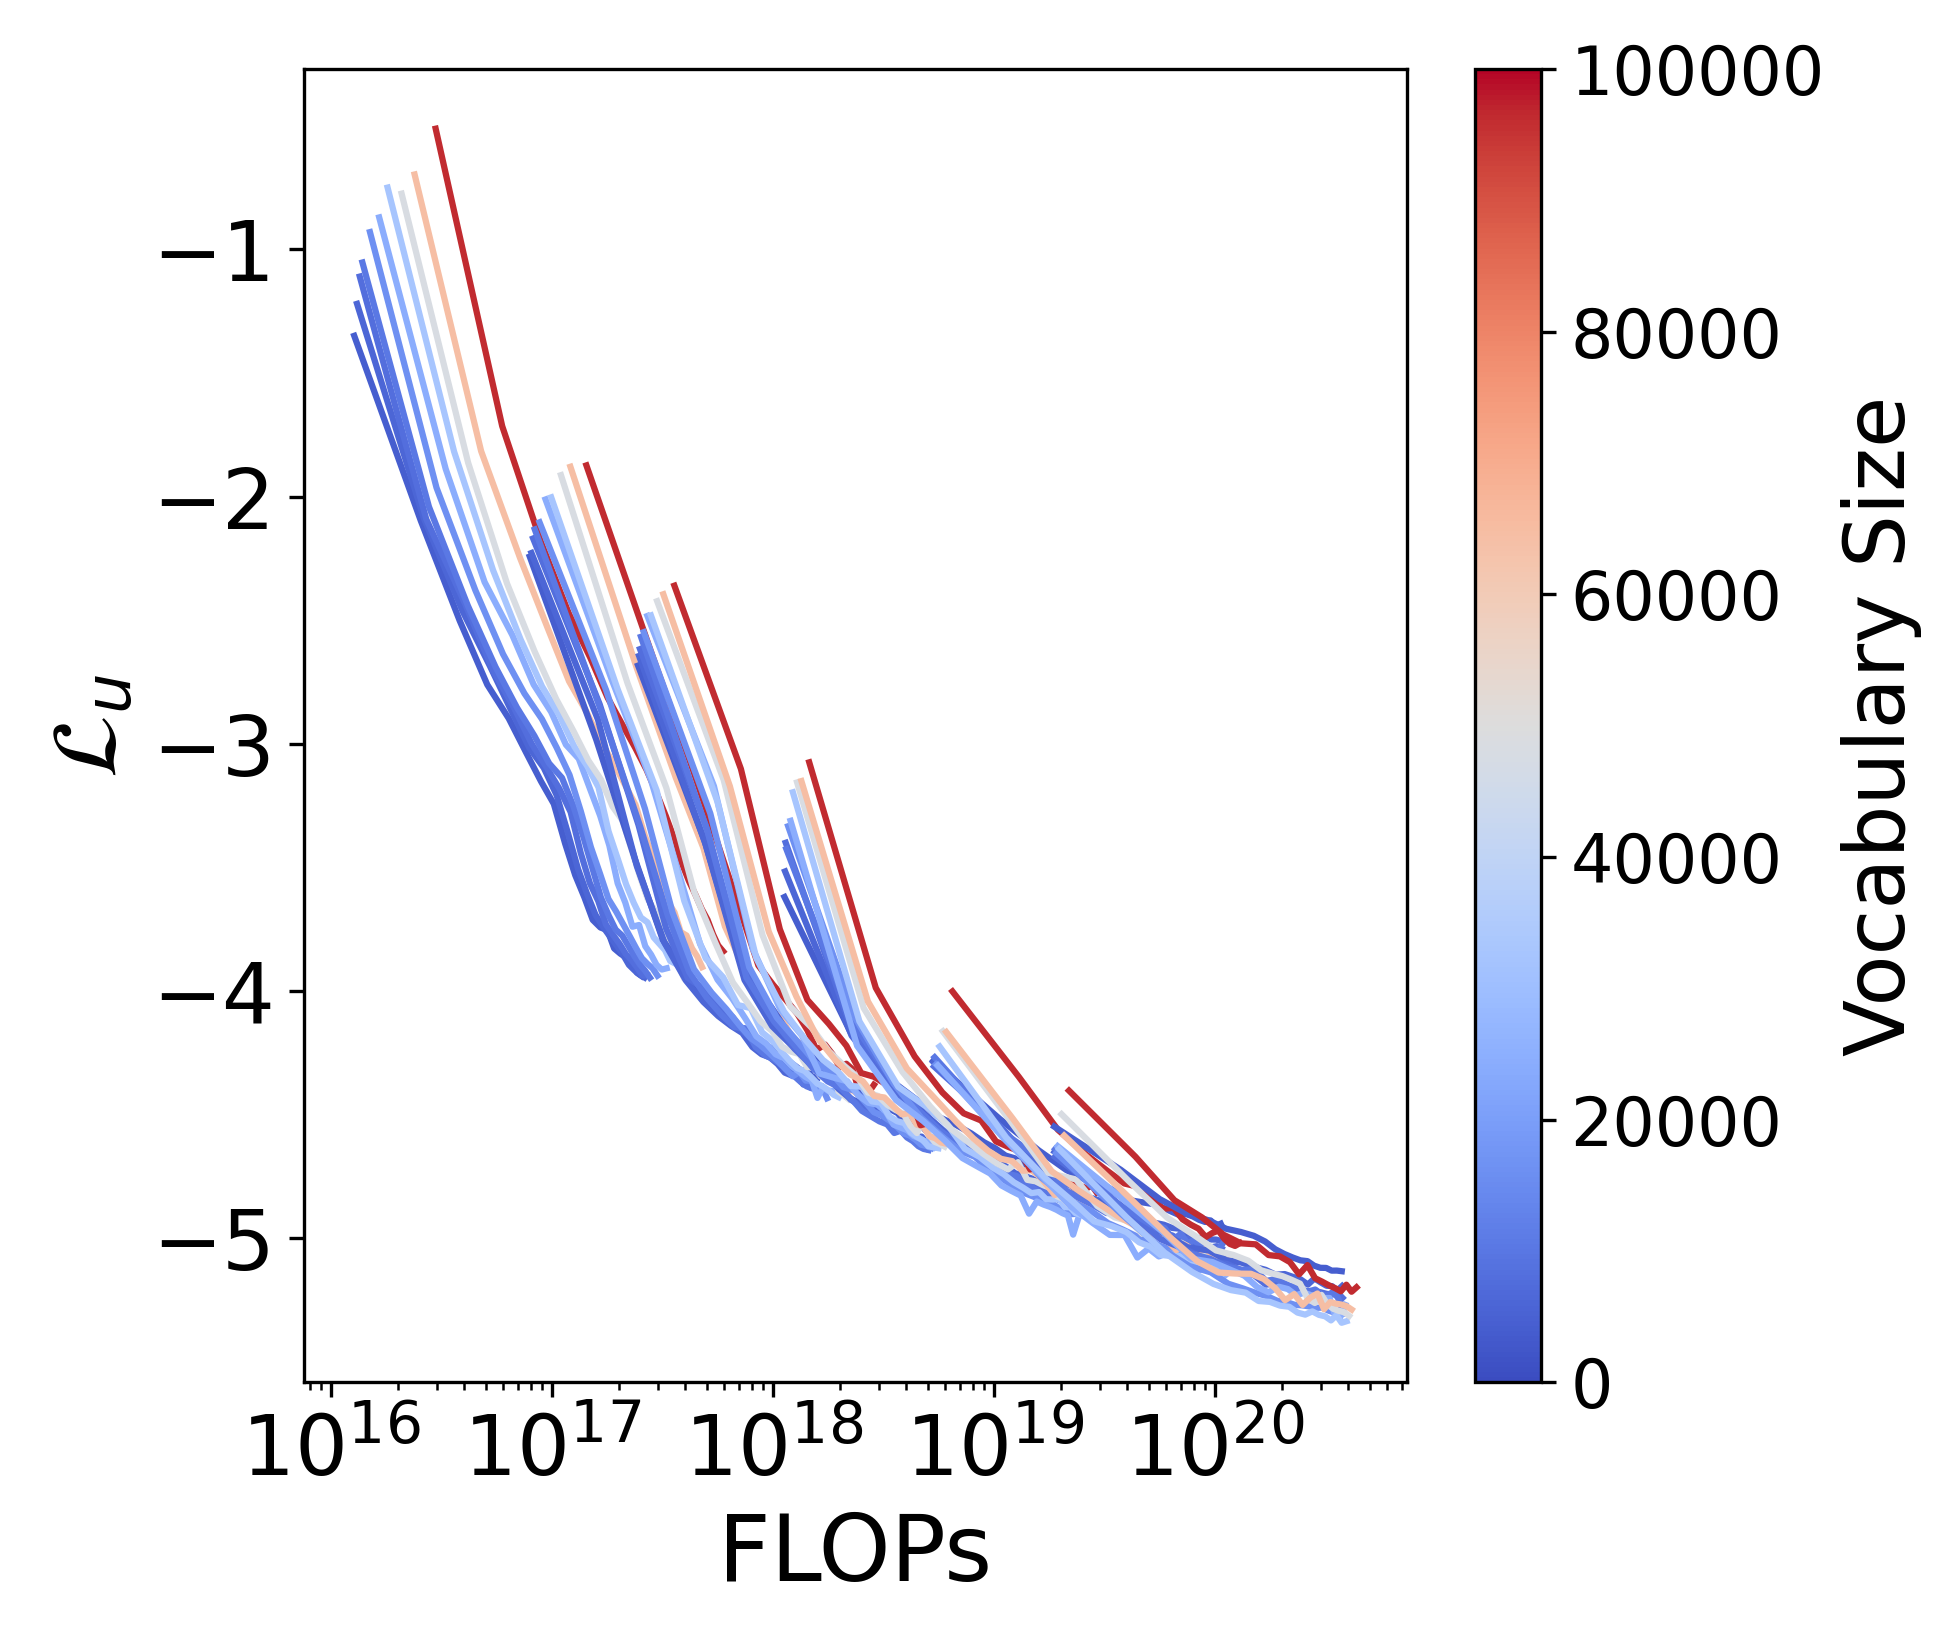
\includegraphics[width=0.45\textwidth]{figures/slim_N_lt_1b_plot_intepolated.png}
\caption{Training curves of the experiments used in Approach 1 (\autoref{sec:isoflops}) and Approach 3 (\autoref{sec:parametric}). We train models with the non-vocabulary parameters fixed and vocabulary sizes varying from 4K to 96K.}
\label{fig:empirical_data}
\vspace{-6mm}
\end{wrapfigure}

\textbf{Setup}\;\;\;\;Given a certain $N_{\rm v}$, the embedding dimension $d$ is fixed,  thus $N_{\rm v}$ increases as $V$ increases. 
For all experiments, we uniformly sample the training data from different domains in the SlimPajama dataset~\citep{soboleva2023slimpajama}. 
All other hyperparameters are fixed with more details in \autoref{append:imple_details}.

\textbf{Fitting}\;\;\;\;We select data points with the minimum $\mathcal{L}_u$ for each FLOP budget, with all runs visualized in \autoref{fig:empirical_data}. These points are the compute-optimal allocation to ($N_{\rm nv}$, $N_{\rm v}$, $H$). Following \citet{kaplan2020scaling} and \citet{hoffmann2022training}, we hypothesize that the optimal vocabulary parameters $N_{\rm v}$ meet a power law w.r.t. the FLOPs $C$, just like the non-vocabulary parameters and the amount of training data. Specifically, $N_{\rm nv}=k_1C^{\alpha_1}$,$N_{\rm v}=k_2C^{\alpha_2}$ and $H=k_3C^{\alpha_3}$. As model size and training data should be scaled equally for compute-optimal training~\citep{hoffmann2022training}, we set  $\alpha_1=\alpha_3$. As our new attribute $V$ significantly increases the number of possible experimental configurations, we employ interpolation across data points to obtain more configurations cheaply. The details of the fitting are in \autoref{append:fitting_tech}.




\begin{figure}[htbp]
\centering
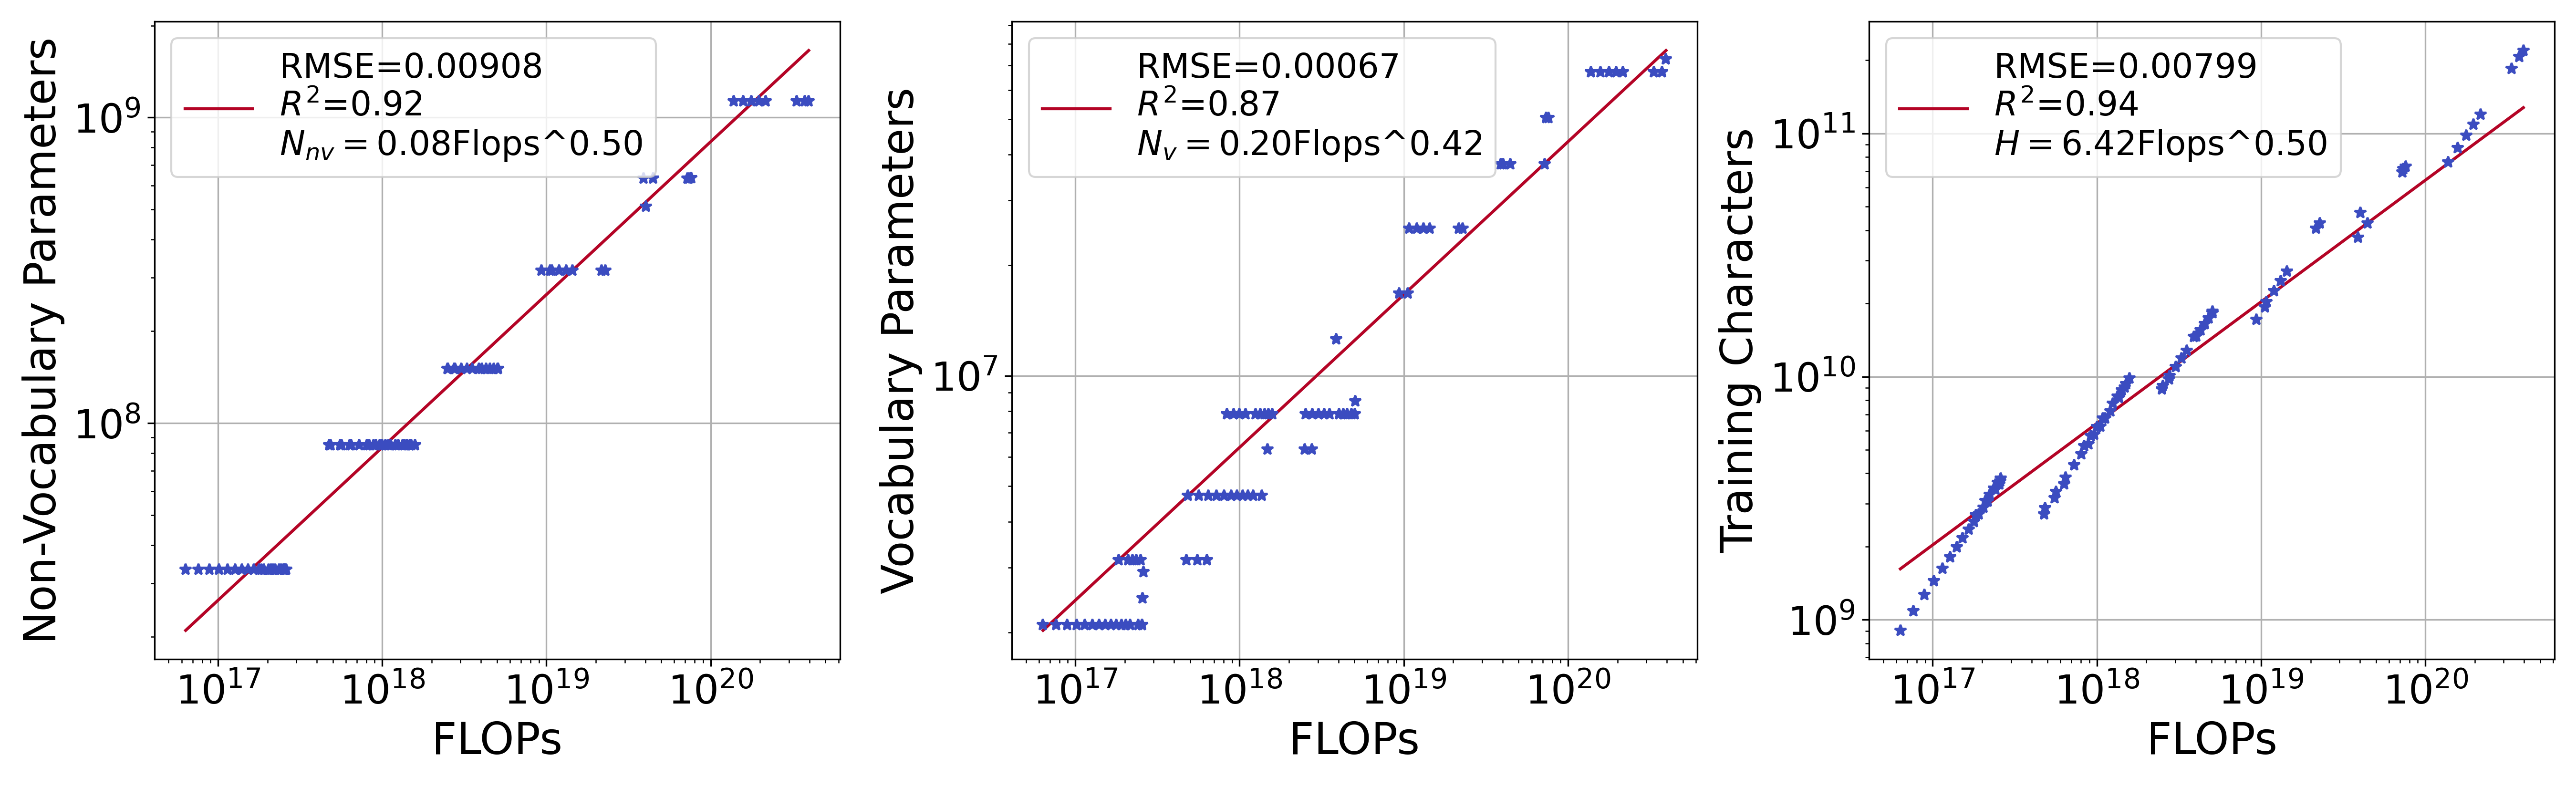
\includegraphics[width=\textwidth]{figures/fit_results.png}
\caption{Fitting results of the Approach 1. Blue stars denote the selected data points where the combination ($N_{\rm nv}$, $N_{\rm v}$, $H$) reaches the lowest loss given various FLOPs budgets. We find power law fits with respect to the optimal non-vocabulary parameters, vocabulary parameters, and the number of training characters, respectively.
}
\label{fig:all_fit}
\end{figure}

\textbf{Results and Usage}\;\;\;\;
In \autoref{fig:all_fit}, we display the fitted power laws: $N_{\rm nv}=0.08*C^{0.50}$, $N_{\rm v}=0.20*C^{0.42}$ and $H=6.42*C^{0.50}$, where $C$ is the FLOPs budget.The low $\rm RMSE$ and high $R^2$ values indicate the strength of our fit. Given a certain FLOPs budget, we can utilize the aforementioned relationships to obtain the optimal allocation ($N_{\rm nv}$, $N_{\rm v}$, $H$). We also draw the following conclusions: \textbf{(1) LLMs are data-hungry.} Compared to the non-vocabulary parameters $N_{\rm nv}$, practitioners should allocate more compute to the training data~\citep{xue2024repeat,muennighoff2024scaling}. \textbf{(2) Vocabulary parameters scale in a power-law relation with FLOPs ($N_{\rm v} \propto C^{0.42}$).} As models become more computationally intensive, a larger vocabulary enhances the model's ability to understand a more diverse array of text, and thus the vocabulary size is critical to scaling. \textbf{(3) Vocabulary parameters $N_{\rm v}$ should be scaled slower than non-vocabulary parameters $N_{\rm nv}$.} This difference can be seen in their power law exponents, i.e. $\gamma=0.42/0.50=0.84 < 1$. We hypothesize the reason is that: once a sufficiently rich embedding space is present via a large vocabulary, it is more critical to scale non-vocabulary parameters to learn the intricate syntactic and semantic structures of language via Transformer blocks.



\subsection{Approach 2: Derivative-based fast estimation}
\label{sec:derivative}


We propose an alternative approach leveraging insights from the estimation of the FLOPs itself. Prior work~\citep{hoffmann2022training,kaplan2020scaling} usually considers a fixed compute budget in FLOPs and then aims to minimize loss by finding the optimal allocation to model parameters $N$ and training tokens $D$. Here we flip this recipe on its head following recent work~\citep{sardana2023beyond}. We aim to find the minimum FLOPs to achieve a certain loss $\mathcal{L}_u(N_{\rm nv}, V, H)=\ell$ through optimal allocation of the vocabulary size $V$:
\begin{equation}
    V=\mathop{\arg \min}_{V | \mathcal{L}_u(N_{\rm nv},V,H)=\ell} C(N_{\rm nv}, N_v, H).
\end{equation}
By computing the minimum point of FLOPs $C$ with respect to $V$ via derivative:
\begin{equation}
\label{eq:df_dv}
\frac{\partial C}{\partial V}  = 6H \Bigg[ (N_{\rm nv} + Vd) \frac{2a \log(V) + b}{V} + \left[a (\log(V))^2 + b \log(V) + c\right]d \Bigg],
\end{equation}
we can estimate the optimal $V$ under the assumption that it can achieve a certain loss $\mathcal{L}_u(N_{\rm nv}, V, H)=\ell$.
The parameters $a$, $b$ and $c$ can be easily obtained from building $f(V)$ (\autoref{sec:preliminaries}).
In theory, as long as the non-vocabulary parameters $N_{\rm nv}$ are provided, $V$ can be numerically searched via the solution of $\frac{\partial C}{\partial V}=0$.
More details are in \autoref{append:df_dv}.

\textbf{Usage}\;\;\;\;
When the compute allocation is near optimal, the loss exhibits a power-law relationship with respect to the FLOPs budget, as described by the scaling law~\citep{kaplan2020scaling}.
This relationship allows us to use FLOPs  as a reliable proxy for observing the scaling behavior of the optimal vocabulary parameters.
In practice, we can first determine an empirically optimal vocabulary size in a low-cost setting (e.g., finding the compute-optimal vocabulary parameters on a small model). Then, we can scale the optimal vocabulary parameters proportionally based on $\gamma$.
Specifically, we obtain a set of derivative-optimal vocabulary parameters $N_v$ for different non-vocabulary parameters $N_{nv}$, represented as $\left\{(N_{\rm nv}^i, N_{\rm v}^i)| i=1,\cdots,n \right\}$. We then fit the relationship between $N_{\rm nv}$ and $N_{\rm v}$ using the power-law function $N_{\rm v} \propto N_{\rm nv}^\gamma$. This results in the scaling equation:
$N_{\rm v}/N_{\rm v}^0 = (N_{\rm nv}/N_{\rm nv}^0)^\gamma$
where $N_{\rm nv}^0$ is a small model (e.g., 33M), and $N_{\rm v}^0$ is the searched optimal vocabulary parameter.
By combining the $\gamma$  from the derivative and the empirical solution on a small model, we can estimate the optimal vocabulary by:
\begin{align*}
\label{eq:derivative-predict}
N_{\rm v}^{\rm opt}=N_{\rm v}^0*(\frac{N_{\rm nv}}{N_{\rm nv}^0})^\gamma,
\end{align*}
where the scaling proportion $\gamma=0.83$ after our fitting. Consistent with the observation in Approach 1, we find that non-vocabulary parameters should be scaled \textbf{faster} than vocabulary parameters to achieve an optimal allocation.


\subsection{Approach 3: Parametric fit of loss formula}
\label{sec:parametric}
{Finally, we directly predict the loss given the non-vocabulary parameter, vocabulary parameter and the amount of training characters.} Then, the optimal vocabulary configuration can be predicted by finding the minimum point of loss with respect to the vocabulary. Following a classical risk decomposition used in \citet{hoffmann2022training}, we design the vocabulary-dependent loss formula as:
\begin{equation}
\label{eq:loss}
    \mathcal{L}_u = -E + \frac{A_1}{N_{\rm nv}^{\alpha_1}} +\frac{A_2}{N_{\rm v}^{\alpha_2}}+ \frac{B}{D^{\beta}},
\end{equation}
where $D=Hf(V)$.
The first term captures the normalized loss for an ideal generative process. The subsequent terms reflect the effect of the non-vocabulary parameters, vocabulary parameters, and the number of training data on the loss, respectively. $E, A_1, A_2, B, \alpha_1, \alpha_2, \beta$ are learned parameters.

\textbf{Fitting}\;\;\;\;We use the points ($N_{\rm nv}$, $N_{\rm v}$, $H$) collected for experiments in \autoref{sec:isoflops}. Note that we do not only consider the points with the lowest loss for each FLOP budget as we want to predict loss for any combination of ($N_{\rm nv}$, $N_{\rm v}$, $H$). We add the constraint $\alpha_1=\beta$ following \citet{muennighoff2024scaling}. We also filter out points with very small FLOPs following \citet{hoffmann2022training}. 
Fitting yields $A_1=1.831$, $A_2=0.196$, $B=2.124$, $E=5.533$, $\alpha_1=\beta=0.447$, $\alpha_2=0.671$. The detailed fitting process is written in \autoref{append:fitting_tech}.

\textbf{Usage}\;\;\;\;After fitting the parameters in \autoref{eq:loss}, the optimal vocabulary size can be obtained by finding the lowest loss w.r.t the vocabulary size, with a constraint of FLOPs budget. For example, given $N_{\rm nv}$ and FLOPs budget $C$ , by replacing $[Hf(V)]$ with $C/(6(N_{\rm nv}+N_v))$ and finding the solution of $\frac{\partial \mathcal{L}_u}{\partial V}=0$ via numerical search, we can get the prediction. The details of $\frac{\partial \mathcal{L}_u}{\partial V}$ is written in \autoref{append:dloss_dv}. 
Note that all of the proposed approaches can be used in optimally allocating  ($N_{\rm nv}, N_{\rm v}, H$) altogether, while Approach 3 is more flexible in predicting the locally optimal $N_{\rm v}$ when ($N_{\rm nv}$, $H$) are not following the Chinchilla's law \citep{hoffmann2022training}, \textit{i.e.} equally-scaled law. The reason is that the loss formula in Approach 3 does not only considers the combinations  ($N_{\rm nv}, N_{\rm v}, H$) which reach the optimal given a certain training budget. {By fixing $N_{\rm nv}$ and varying $C$ in Approach 3, we can predict the locally optimal vocabulary size with different amount of training characters}. This property makes Approach 3 more valuable, since modern LLMs \citep{touvron2023llama,team2024gemma,allal2023santacoder,almazrouei2023falcon,deepseekllm2024} usually leverage overly sufficient training data to build powerful models with relatively low inference costs. 

\begin{figure}[t]
\centering
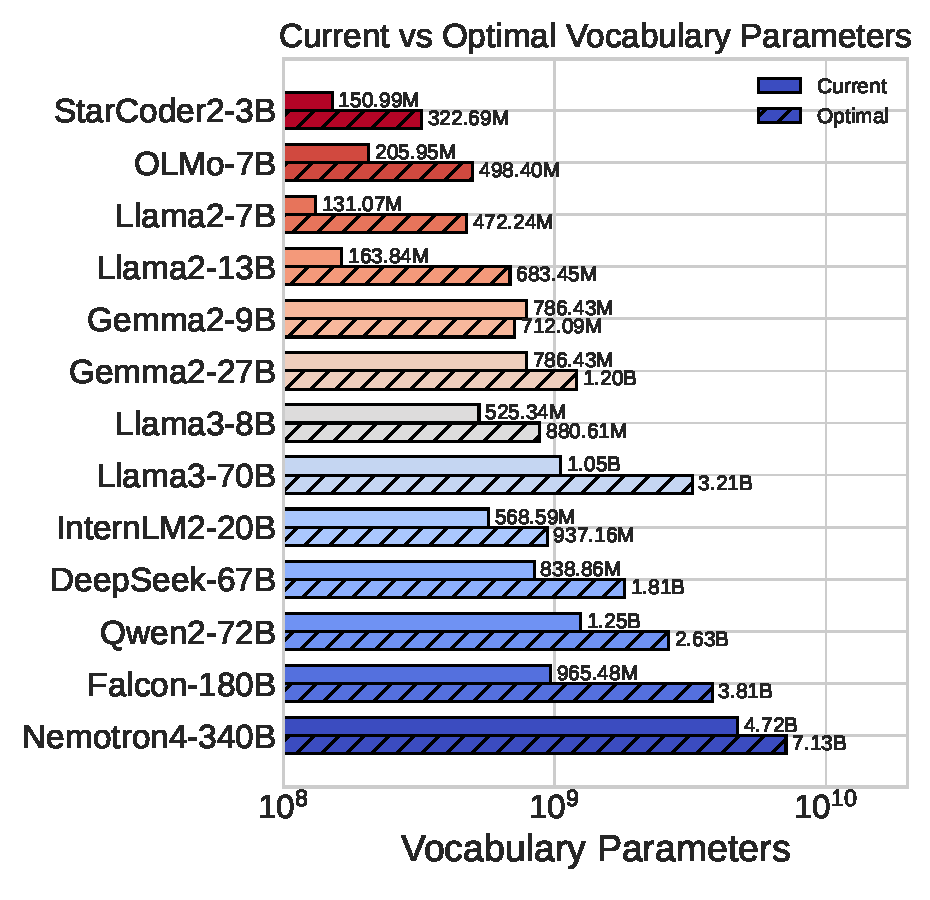
\includegraphics[width=.52\textwidth]{figures/public_llms_optimal_vocab_parameters_comparsion_v7.pdf}
\caption{Vocabulary parameters of popular LLMs and predicted optimal vocabulary parameters at \textbf{their reported number of training tokens}, as determined by our Approach 3 (\autoref{sec:parametric}). Here we consider the practical scenarios where parameters and training data are not necessarily equally scaled.
As illustrated, the vocabulary parameters remain predominantly underestimated. With the exception of Gemma2-9B, all models allocate a smaller vocabulary parameter count than our prediction.}
\label{fig:public_llms}
\end{figure}

In \autoref{fig:public_llms}, we remove the assumption \citep{hoffmann2022training} for the practical reason that the parameters and training data are not equally scaled. Then, we predict the locally optimal vocabulary parameters. It can be observed that the allocation of vocabulary parameters are typically under-estimated.
